\documentclass[12pt, openany]{report}
\usepackage[utf8]{inputenc}
\usepackage[T1]{fontenc}
\usepackage{amsmath,amsfonts,amssymb}
\usepackage{amssymb}
\usepackage{multicol}
\usepackage[a4paper,left=2.5cm,right=2.5cm,top=2.5cm,bottom=2.5cm]{geometry}
\usepackage[english]{babel}
\usepackage{libertine}
\usepackage{graphicx}
\usepackage{wrapfig}
\usepackage{float}
\usepackage{enumitem}
\usepackage{pythonhighlight}
\usepackage[]{titletoc}
\usepackage{empheq}
\usepackage{titlesec}
\usepackage{mathpazo}
\usepackage{xfrac}
\usepackage{textcomp}
\usepackage{mathtools}
\usepackage{caption}
\usepackage{tabularray}
\usepackage{subcaption}
\usepackage[bottom]{footmisc}
\usepackage{pdfpages}
\usepackage{tabularx}
\usepackage[skins]{tcolorbox}
\titleformat{\chapter}[display]
  {\normalfont\bfseries}{}{0pt}{\Huge}
\usepackage{hyperref}
\newcommand{\hsp}{\hspace{20pt}}
\newcommand{\HRule}{\rule{\linewidth}{0.5mm}}
\newcommand\independent{\protect\mathpalette{\protect\independenT}{\perp}}
\def\independenT#1#2{\mathrel{\rlap{$#1#2$}\mkern2mu{#1#2}}}

% Define a new tcolorbox style with a red border and transparent interior
\tcbset{
    redbox/.style={
        enhanced,
        colframe=red,
        colback=white,
        boxrule=1pt,
        sharp corners,
        before skip=10pt,
        after skip=10pt,
        box align=center,
        width=\linewidth-2pt, % Adjust the width dynamically
    }
}
\newcommand{\boxedeq}[1]{
\begin{tcolorbox}[redbox]
    \begin{align}
        #1
    \end{align}
\end{tcolorbox}
}

\begin{document}


\begin{titlepage}
    \begin{sffamily}
    \begin{center}
        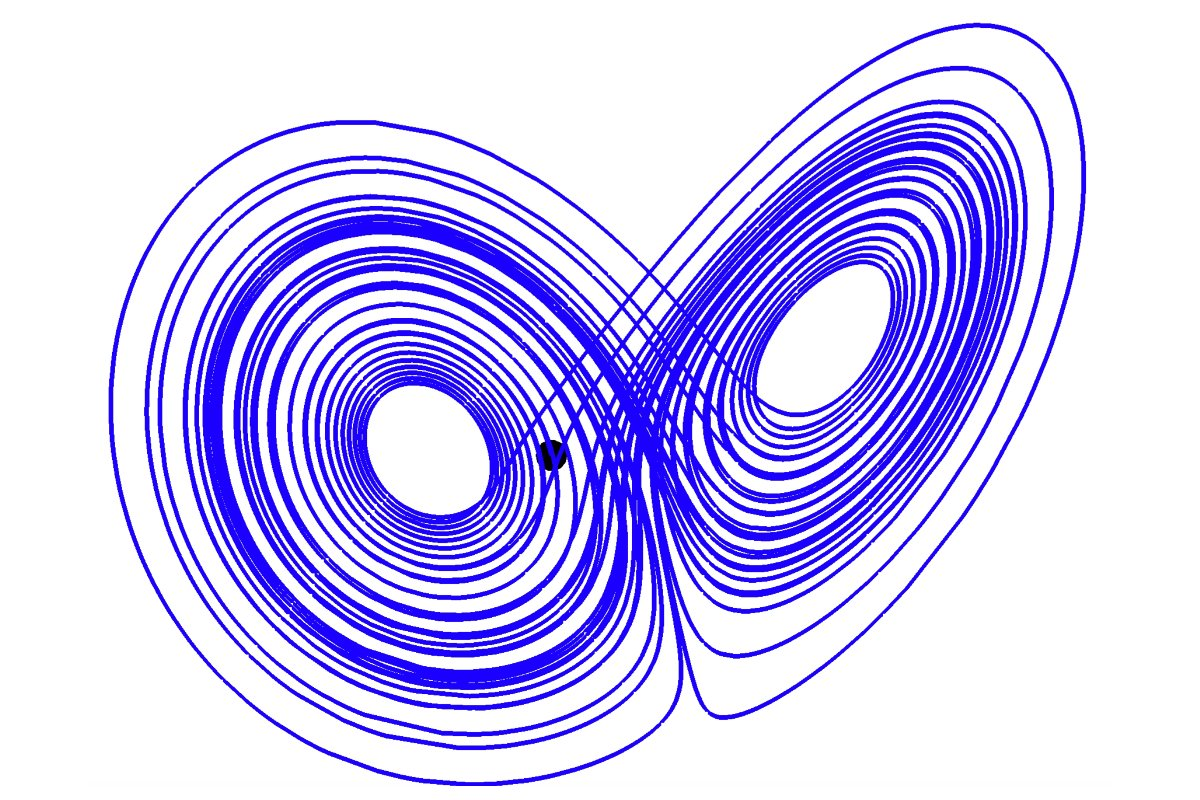
\includegraphics[scale=0.25]{img/page_de_garde.png} \\[1cm]
        \HRule \\[0.4cm]
        { \huge \bfseries LINMA2370 Modelling and Analysis of Dynamical Systems \\[0.4cm] }
    
        \HRule \\[1.5cm]
        \textsc{\LARGE Simon Desmidt\\Issambre L'Hermite Dumont}\\[1cm]
        \vfill
        \vspace{2cm}
        {\large Academic year 2024-2025 - Q1}
        \vspace{0.4cm}
         
        
\includegraphics[width=0.15\textwidth]{img/epl.png}
        
        UCLouvain\\
    
    \end{center}
    \end{sffamily}
\end{titlepage}

\setcounter{tocdepth}{1}
\tableofcontents

\chapter{Methodology}

\section{Theoretically}
% The modelisation and the analysis of a dynamical system requires to follow a set of steps, in order to have a clear overview of the system.\\

% Firstly, we can draw the system that we want to model, at rest and in the movement that we want to analyse.\\

% After that, we will model the system and its dynamics with a set of ODE.\\

% And finally, we can analyse the system and its modelisation, in order to understand it. For example we can analyse the quantitive and qualitative behaviour of the system. Its equilibrium point(s), and the eigenvalues of the problems that will show the mode/focus where the system tends to.\\
Steps to follow, in order to have an overview of the system:
\begin{itemize}
    \item draw the system at rest/in useful mvt
    \item model the system with ODE's
    \item solve ODE system
    \item analyse the eigenvalues and how the system reacts
    \item deduce a qualitative/quantitative behaviour of the system
\end{itemize}

\section{Example}
Tacoma Narrows Bridge

\chapter{Terminology and notation}


\end{document}